%%%%%%%%%%%%%%%%%%%%%%%%%%%%%%%%%%%%%%%%%%%%%%%%%%%%%%%%%%%%%%%%%
%
%   Template para monografia de TCC-2018 - versao 1.0.alfa
%
%%%%%%%%%%%%%%%%%%%%%%%%%%%%%%%%%%%%%%%%%%%%%%%%%%%%%%%%%%%%%%%%%
%%
%% Este template utiliza o modelo mantido pela abnt e foi baseado 
%% no abtex2-modelo-trabalho-academico.tex, v-1.9.6 laurocesar
%% Copyright 2012-2016 by abnTeX2 group at http://www.abntex.net.br/ 
%%
% -------------------------------------------------------------------
%% This work may be distributed and/or modified under the conditions 
%% of the LaTeX Project Public License, either version 1.3 of this 
%% license or (at your option) any later version. The latest version 
%% of this license is in http://www.latex-project.org/lppl.txt
%% and version 1.3 or later is part of all distributions of LaTeX
%% version 2005/12/01 or later.
%%
%% This work has the LPPL maintenance status `maintained'.
%% 
%% The Current Maintainer of this work is the abnTeX2 team, led
%% by Lauro César Araujo. Further information are available on 
%% http://www.abntex.net.br/
%%
%% This work consists of the files abntex2-modelo-trabalho-academico.tex,
%% abntex2-modelo-include-comandos and abntex2-modelo-references.bib
% -------------------------------------------------------------------
%%
%% Modelo de Monografia em conformidade com ABNT NBR 14724:2011
%%
%%%%%%%%%%%%%%%%%%%%%%%%%%%%%%%%%%%%%%%%%%%%%%%%%%%%%%%%%%%%%%%%%
%%
%% ATENÇAO para as opções:
%%
%% para modo rascunho, sem páginas brancas, use: 
%% openany, oneside, nopartblankpage
%%
%% para modo normal, com tudo que ABNT exige, use:  
%% openright, twoside, partpageblank
%%

\documentclass[
	% -- opções da classe memoir --
	12pt,			% tamanho da fonte
	openany,		% capítulos começam em qq página (isso elimina várias pág brancas)
	%openright,		% capítulos começam em pág ímpar (insere página vazia caso preciso)
	oneside,		% considera impressão de um só lado (gera menos pág brancas)
	%twoside,		% para impressão em recto e verso. Oposto a oneside
	a4paper,		% tamanho do papel. 
	% -- opções da classe abntex2 --
	%chapter=TITLE,		% títulos de capítulos convertidos em letras maiúsculas
	%section=TITLE,		% títulos de seções convertidos em letras maiúsculas
	%subsection=TITLE,	% títulos de subseções convertidos em letras maiúsculas
	%subsubsection=TITLE,% títulos de subsubseções convertidos em letras maiúsculas
	% -- opções do pacote babel --
	english,		% idioma adicional para hifenização
	%french,		% idioma adicional para hifenização
	%spanish,		% idioma adicional para hifenização
	%portuges		% o último idioma é o principal do documento
	brazil			% o último idioma é o principal do documento
	]{abntex2}


% ------------------------------------------------------------------------
%   Componente do template para monografia de TCC-2018 - versao 1.0.alfa
% ------------------------------------------------------------------------

%------------ Pacotes básicos 
\usepackage{lmodern}			% Usa a fonte Latin Modern			
\usepackage[T1]{fontenc}		% Selecao de codigos de fonte.
\usepackage[utf8]{inputenc}		% Codificacao do documento (conversão automática dos acentos)
\usepackage{lastpage}			% Usado pela Ficha catalográfica
\usepackage{indentfirst}		% Indenta o primeiro parágrafo de cada seção.
\usepackage{color}			% Controle das cores
\usepackage{graphicx}			% Inclusão de gráficos
\usepackage{microtype} 			% para melhorias de justificação
		
%------------ Pacotes adicionais
\usepackage{blindtext}			% para geração de dummy text

%------------ Pacotes de citações
\usepackage[brazilian,hyperpageref]{backref}	% Paginas com as citações na bibl
\usepackage[alf]{abntex2cite}		% Citações padrão ABNT
\usepackage{pdfpages}			% Saida em pdf

%------------ Comandos úteis
\newcommand{\aspas}[1]{``#1''}

% ----------- CONFIGURAÇÕES DE PACOTES

% Configurações do pacote backref
% Usado sem a opção hyperpageref de backref
\renewcommand{\backrefpagesname}{Citado na(s) página(s):~}
% Texto padrão antes do número das páginas
\renewcommand{\backref}{}
% Define os textos da citação
\renewcommand*{\backrefalt}[4]{
	\ifcase #1 %
		Nenhuma citação no texto.%
	\or
		Citado na página #2.%
	\else
		Citado #1 vezes nas páginas #2.%
	\fi}%
% ---

% Espaçamentos entre linhas e parágrafos 
% O tamanho do parágrafo é dado por:
\setlength{\parindent}{1.3cm}
% Controle do espaçamento entre um parágrafo e outro:
\setlength{\parskip}{0.2cm}  % tente também \onelineskip

% compila o indice
\makeindex

% ----------------------------------------------------
% Configurações de aparência do PDF final
% ----------------------------------------------------

% alterando o aspecto da cor azul
\definecolor{blue}{RGB}{41,5,195}

% informações do PDF
\makeatletter
\hypersetup{
     	%pagebackref=true,
		pdftitle={\@title}, 
		pdfauthor={\@author},
    	pdfsubject={\imprimirpreambulo},
	    pdfcreator={LaTeX with abnTeX2},
		pdfkeywords={abnt}{latex}{abntex}{abntex2}{trabalho acadêmico}, 
		colorlinks=true,       		% false: boxed links; true: colored links
    	linkcolor=blue,          	% color of internal links
    	citecolor=blue,        		% color of links to bibliography
    	filecolor=magenta,      		% color of file links
		urlcolor=blue,
		bookmarksdepth=4
}
\makeatother

% ----------------------------------------------------
% Comandos para geração de itens textuais 
% ----------------------------------------------------

\newcommand{\imprimirfichacatalografica}{

\begin{fichacatalografica}
	\sffamily
	\vspace*{\fill}					% Posição vertical
	\begin{center}					% Minipage Centralizado
	\fbox{\begin{minipage}[c][8cm]{13.5cm}		% Largura
	\small
	
	\hspace{1cm} \imprimirautor\\

	\begingroup
        \leftskip4em
        \rightskip\leftskip
	
	\imprimirtitulo  / \imprimirautor. -- \imprimirlocal, \imprimirdata.
	
	\pageref{LastPage} p. : il. (algumas color.) ; 30 cm.\\
	
	\imprimirorientadorRotulo~\imprimirorientador\\
	
	%\imprimirtipotrabalho~--~\imprimirinstituicao, \imprimirdata.\\
	Monografia para trabalho de conclusão de curso (graduação)~--~Instituto Federal 
	de Educação, Ciência e Tecnologia de Minas Gerais, Ciência da Computação, 
	Formiga, \imprimirdata.\\
	
	1. Palavra-chave1.
	2. Palavra-chave2.
	3. Palavra-chave3.
	I. \imprimirorientador.
	II. Instituto Federal de Educação, Ciência e Tecnologia de Minas Gerais.
	III. Ciência da Computação.
	IV. \imprimirtitulo 			
        \par
        \endgroup
	\end{minipage}}
	\end{center}
\end{fichacatalografica}

}

\newcommand{\imprimirerrata}{

\begin{errata}
Exemplo de errata\\[1cm]

FERRIGNO, C. R. A. \textbf{Tratamento de neoplasias ósseas apendiculares com
reimplantação de enxerto ósseo autólogo autoclavado associado ao plasma
rico em plaquetas}: estudo crítico na cirurgia de preservação de membro em
cães. 2011. 128 f. Tese (Livre-Docência) - Faculdade de Medicina Veterinária e
Zootecnia, Universidade de São Paulo, São Paulo, 2011.

\begin{table}[htb]
\center
\footnotesize
\begin{tabular}{|p{1.4cm}|p{1cm}|p{3cm}|p{3cm}|}
  \hline
   \textbf{Folha} & \textbf{Linha}  & \textbf{Onde se lê}  & \textbf{Leia-se}  \\
    \hline
    1 & 10 & auto-conclavo & autoconclavo\\
   \hline
\end{tabular}
\end{table}

\end{errata}

}

\newcommand{\imprimirfolhadeaprovacao}[1]{

\begin{folhadeaprovacao}
  \begin{center}
   {\ABNTEXchapterfont\large\imprimirautor}

   \vspace*{\fill}\vspace*{\fill}
   \begin{center}
     \ABNTEXchapterfont\bfseries\Large\imprimirtitulo
   \end{center}
   \vspace*{\fill}
    
   \hspace{.45\textwidth}
   \begin{minipage}{.5\textwidth}
       \imprimirpreambulo
   \end{minipage}%
   \vspace*{\fill}        
   \end{center}
   
   Trabalho aprovado em {#1}.
   
   \vspace{1cm}
   \hspace{4cm} BANCA EXAMINADORA    

   \assinatura{\textbf{\imprimirorientador} \\ Orientador} 
   \assinatura{\textbf{Fulano} \\ Convidado 1}
   \assinatura{\textbf{Sicrano} \\ Convidado 2}
   %\assinatura{\textbf{Professor} } %\\ Convidado 3}
   %\assinatura{\textbf{Professor} } %\\ Convidado 4}
      
   \begin{center}
    \vspace*{0.5cm}
    {\large\imprimirlocal}
    \par
    {\large\imprimirdata}
    \vspace*{1cm}
  \end{center}
  
\end{folhadeaprovacao}

}

	

\graphicspath{{./figuras/}}   	% pasta contendo todas as figuras

\nopartblankpage  		% elimina páginas em branco
% \partpageblank		% permite páginas em branco

% ----------------------------------------------------
% Informações de dados para CAPA e FOLHA DE ROSTO
% ----------------------------------------------------

\titulo{Título do TCC}
\autor{Lucas Mateus Fernandes}
\local{Formiga - MG}
\data{2023}
\orientador{Fernando Paim Lima}
% \coorientador{Felipe Augusto Lima Reis}
\instituicao{%
  Instituto Federal de Educação, Ciência e Tecnologia de Minas Gerais \par
  Campus Formiga \par
  Ciência da Computação
  }
\tipotrabalho{Monografia}

% O preambulo deve conter o tipo do trabalho, o objetivo, o nome da instituição e a área de concentração 
%\preambulo{Monografia do trabalho de conclusão de curso apresentado ao Instituto Federal Minas Gerais - Campus Formiga, como requisito parcial para a obtenção do título de Bacharel em Ciência da Computação.}


\preambulo{Proposta de projeto do Trabalho de Conclusão de Curso do Curso de Bacharelado em Ciência da Computação, IFMG – Campus Formiga.}

    
% ----------------------------------------------------
% INÍCIO DO DOCUMENTO
% ----------------------------------------------------

\begin{document}

%\selectlanguage{portuges}
\selectlanguage{brazil}

\frenchspacing  % retira espaço extra obsoleto entre as frases.

%-----------------------------------------------------
% ELEMENTOS PRÉ-TEXTUAIS
%-----------------------------------------------------
% \pretextual

\imprimircapa

\imprimirfolhaderosto*  % o comando com * indica que haverá ficha bibliográfica

%------------- Ficha catalográfica
% São os ``Dados internacionais de catalogação-na-publicação''.
% Escolha uma das opções: usar página pdf pronta (gerada pela biblioteca?!)
% ou gerar a página com o comando \imprimirfichacatalografica. 
% (Mais detalhes no preludio e documentacao do pacote abntex2.)
%
% \begin{fichacatalografica}
%     \includepdf{ficha_catalografica.pdf}
% \end{fichacatalografica}
\imprimirfichacatalografica

%------------ Errata (se houver)
% Modifique o comando \imprimirerrata no preludio e use esse comando
%\imprimirerrata

%------------ Folha de aprovação
% É um elemento obrigatório da NBR 14724/2011 (seção 4.2.1.3). 
% Você pode utilizar a página modelo até a aprovação do trabalho. 
% Após isso, gere uma página com a imagem da folha assinada pela banca,
% comente o comando \imprimirfolhadeaprovacao e use o \includepdf 
\imprimirfolhadeaprovacao{06 de junho de 2018}
% \includepdf{folhadeaprovacao_final.pdf}

%------------ Dedicatória
\begin{dedicatoria}
   \vspace*{\fill} \centering \noindent 
   \textit{ Este trabalho é dedicado a tudo e todos, exceto os cachorros de rua.} 
   \vspace*{\fill}
\end{dedicatoria}

%------------ Agradecimentos
\begin{agradecimentos}
  Gostaria de agradecer meus pais por tudo que fizeram e
  aos meus professores pela paciência que tiveram.
\end{agradecimentos}


%------------ Epígrafe
\begin{epigrafe}
   \vspace*{\fill}
   \begin{flushright}
	\textit{\aspas{Nunca atribua à malícia/maldade o que pode ser adequadamente explicado pela estupidez.}
	(Navalha de Hanlon) }
   \end{flushright}
\end{epigrafe}

%------------ RESUMOS
\setlength{\absparsep}{18pt} % ajusta o espaçamento dos parágrafos do resumo

% resumo em português
\begin{resumo}
 A escrita da monografia é um problema clássico no Trabalho de Conclusão de Curso (TCC).
 Aqui é o lugar onde o autor explica brevemente o conteúdo do seu trabalho. Para usar este
 template é necessário instalar alguns pacotes do LaTeX, particularmente o abntex2. O pacote
 blindtex não é realmente necessário, serve apenas para gerar lero-lero neste exemplo.
 
 \textbf{Palavras-chave}: Monografia, LaTeX, TCC.
\end{resumo}

% resumo em inglês
\begin{resumo}[Abstract]
 \begin{otherlanguage*}{english}
  The writing of the monograph is a classic problem in the Course Conclusion Work.
  Here is where the author briefly explains the content of his work.
 
 \textbf{Keywords}: Monograph, LaTeX.
 \end{otherlanguage*}
\end{resumo}

% Consulte o manual da classe abntex2 para maiores 
% orientações sobre os seguintes tópicos:

%------------ Lista de ilustrações
\pdfbookmark[0]{\listfigurename}{lof}
\listoffigures*
\cleardoublepage

%------------ Lista de tabelas

%------------ Lista de abreviaturas e siglas

%------------ Lista de símbolos

%------------ Sumario
\pdfbookmark[0]{\contentsname}{toc}
\tableofcontents*
\cleardoublepage

% ----------------------------------------------------------
% ELEMENTOS TEXTUAIS
% ----------------------------------------------------------
\textual
% ----------------------------------------------------------
\chapter{Introdução}
% ----------------------------------------------------------


O \ac{TAF} é uma das etapas comuns em concursos públicos para provimento de cargos em carreiras relacionadas à área de segurança pública. Sua finalidade é atestar a capacidade do indivíduo em desempenhar funções específicas do cargo, por meio de parâmetros preestabelecidos em edital. Os exercícios avaliados comumente são: barra fixa, salto de impulsão horizontal, corrida de 12 km ou 2.400 m, natação e flexão abdominal. Entretanto, esta é uma etapa muito negligenciada e acaba sendo responsável por um alto índice de reprovação \cite{reprovaTAF}.

Embora seja possível encontrar ferramentas computacionais que utilizam o processamento de imagens para auxiliar no aprimoramento de movimentos em diversas atividades físicas, como mostrado no trabalho de Franke (\citeyear{vcBicicleta}), Pádua (\citeyear{vcFutebol}) e Paulichen (\citeyear{futebolTatica}), é incomum encontrar ferramentas analíticas tecnológicas que auxiliem na melhoria ou indiquem a execução correta do movimento de barra fixa. No entanto, ainda existem poucas ferramentas computacionais analíticas que visam aprimorar exercícios exigidos durante o \ac{TAF}, possivelmente devido a questões de investimento/retorno financeiro ou outras justificativas.

A flexão de braços na barra fixa, também conhecida como movimento de barra fixa, é uma atividade física que tem como objetivo avaliar a resistência e a força dos músculos do tronco e dos membros superiores. Esse exercício é amplamente utilizado em diversos contextos, principalmente por sua facilidade de aplicação, baixo custo e alta reprodutibilidade \cite{barraFixa}. De acordo com o Governo da Paraíba, a realização do movimento de barra fixa foi identificada como o principal motivo de reprovação durante o \ac{TAF} nos concursos de 2018 para a Polícia Militar da Paraíba (PMPB) e o Corpo de Bombeiros Militar da Paraíba (PMPB) \cite{barraTAF}.

Portanto, este trabalho visa à criação de uma ferramenta que contribua para o aperfeiçoamento do movimento de barra fixa, proporcionando um feedback visual com informações da análise autonoma da angulação dos cotovelos e dos quadris, quantidade de barras executadas e o atendimento aos critérios estabelecidos nos \ac{TAF}s.
% ----------------------------------------------------------
\chapter{Fundamentação Teórica}
% ----------------------------------------------------------

Neste capítulo são mostrados os principais fundamentos necessários para entender os
conceitos abordados no presente trabalho.

\section[TAF]{TAF}


O Teste de Aptidão Física (TAF). é uma etapa comum em concursos públicos para provimento de cargos em carreiras relacionadas a área de segurança pública. Seu objetivo é atestar a capacidade do indivíduo em desempenhar funções específicas do cargo por meio da avaliação de determinados exercícios. A avaliação é embasada em exercícios e parâmetros pré estabelecidos em edital como por exemplo: quantidade de repetições de um determinado movimento para o exercício de barra fixa ou flexão abdominal, tempo gasto para translocação em uma determinada distancia nas corridas de 12km, 2.400m ou natação, ou até mesmo a distância percorrida durante o salto de impulsão horizontal.


\section[Barra Fixa]{Barra Fixa}

Nos ultimos 4 anos é possivel ver uma série de concursos publicos que avaliam o movimento de barra fixa no teste de aptidão física (TAF) como por exemplo:
Concurso público para admissão ao curso de formação de soldados bombeiros militar do quadro de praças (qp-bm) e do quadro de praças especialistas – (qpe-bm) do corpo de bombeiros militar de minas gerais para o ano de 2020.\cite{eCBMG2018};
Concurso público para admissão ao curso de formação de soldados do quadro de praças especialistas da polícia militar de minas gerais.\cite{ePMMG2021};
Concurso público para o provimento de vagas nos cargos de delegado de polícia federal, agente de polícia federal, escrivão de polícia federal e papiloscopista policial federal.\cite{ePF2021};
Concurso público para provimento de cargos da carreira de agente de segurança penitenciário/policial penal do quadro de pessoal da secretaria de estado de justiça e segurança\cite{ePP2021}.

O teste de flexão em barra fixa ou teste dinâmico de barra fixa sofre algumas divergencias de acordo com o edital porem os principios do movimento são semelhantes.

A barra fixa é instalada a uma altura tal, que o avaliado, mantendo-se pendurado, com os cotovelos em extensão, não tenha contato dos pés com o solo;
A posição da pegada é pronada (dorso da mão voltado para o rosto) e a abertura das mãos corresponde à distância biacromial (largura dos ombros);
Após assumir essa posição, o avaliado deverá elevar o corpo até que o queixo ultrapasse o nível da barra, após o que retornará à posição inicial;
O movimento é repetido tantas vezes quanto possível, sem limite de tempo.
Os cotovelos deverão estar em extensão total para o início de flexão;
É permitido repouso entre um movimento e outro, contudo, o avaliado não poderá tocar os pés no solo;
Não são permitidos movimentos de quadris ou pernas e extensão da coluna cervical como formas de auxiliar na execução da prova.
Somente é contado o número de movimentos completados corretamente.


\section[Visão computacional]{Visão computacional}
Visão computacional é a ciência que estuda e desenvolve tecnologias que permitem extrair características de imagens capturadas por diferentes tipos de sensores e então permitem reconhecer, manipular e processar dados sobre os objetos que compõem a imagem capturada \cite{VisaoComp}.




\cite{visao}






\section[Articulação]{Articulação}
A articulação é a conexão de duas ou mais superfícies ósseas que promovem movimento \cite{articulacao}

\section[Parte Distal]{Parte Distal}
A parte distal é o ponto mais afastado do tronco ou do ponto de origem \cite{distal}.

\section[Origem Muscular]{Origem Muscular}
Origem é a extremidade do músculo que esta fixada a um ponto fixo ou a uma peça ossea que não se desloca \cite{sisMuscular}.

\section[Inserção Muscular]{Inserção Muscular}
Inserção é a extremidade do músculo que esta fixada a um ponto movel ou a uma peça óssea que se desloca \cite{sisMuscular}.

\section[Cadeia Cinemática]{Cadeia Cinemática}
Os termos cadeia cinemática aberta ou fechada, são usados para demonstrar se o segmento mais distal da cadeia está fixado a algum objeto imóvel ou até mesmo o solo \cite{silva2015cinesiologia}.

\subsection[Cadeia Cinemática Aberta]{Cadeia Cinemática Aberta}
Uma cadeia cinemática aberta representa uma situação em que a extremidade do membro não está fixada ao solo ou a algum objeto imóvel e assim, o segmento está livre para se mover\cite{silva2015cinesiologia}.

\subsection[Cadeia Cinemática Fechada]{Cadeia Cinemática Fechada}
Uma cadeia cinemática fechada representa uma situação em que o segmento mais distal da cadeia está fixo ao solo ou a um objeto imóvel \cite{silva2015cinesiologia}.







\section[TERMOS]{Visão computacional}

\section[TERMOS]{Visão computacional}

\section[TERMOS]{DEFINIÇÃO DE TERMOS}






\section[Conceito1]{Primeiro Conceito}

\blindtext

\blindtext[2]

\blindtext

A figura~\ref{fig-tostines} ilustra primeiro material conhecido causador do Efeito Tostines.

\begin{figure}[!htb]
	\centering
	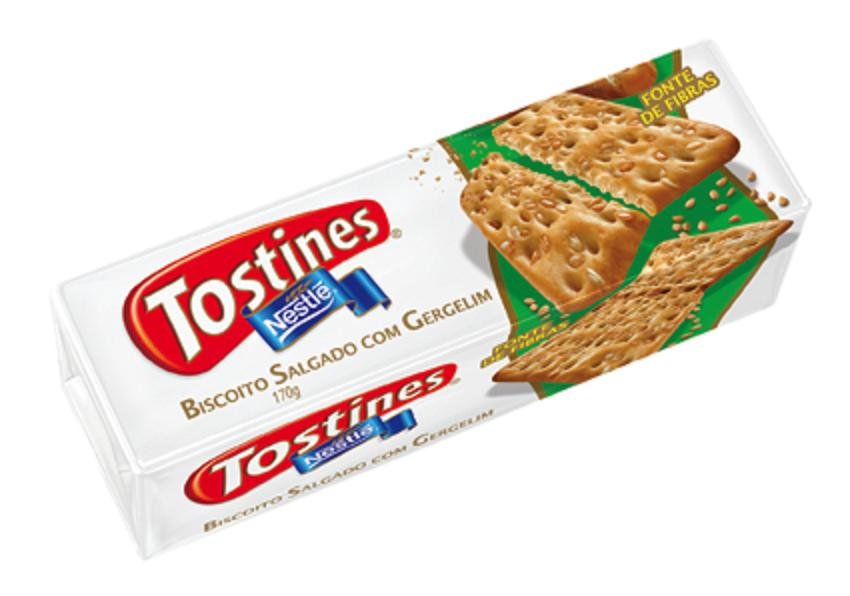
\includegraphics[scale=0.45]{tostines.jpg}
	\caption{Exemplo de objeto causador de Efeito Tostines}
	\label{fig-tostines}
\end{figure}

\blindtext[2]




\section[Conceito2]{Segundo Conceito}

\blindtext

\blindtext[2]

\blindtext
		


% ----------------------------------------------------------
\chapter{Tecnologias e Métodos}
% ----------------------------------------------------------
Neste capítulo são apresentadas a metodologia adotada, juntamente com as ferramentas, bibliotecas e bases de dados que serão utilizadas no desenvolvimento desse trabalho

\section[Metodologia]{Metodologia}


 \begin{itemize}
   \item Realização de revisão da literatura abordando o uso de redes neurais no reconhecimento de pose detection.  
   \item Escolha de base Line ?.
   \item Escolha de uma ferramentas de posedetection para utilização.
   \item Criação das regras de negocio para detecção da execução correta da barra fixa.
   \item Desenvolvimento de uma Ferramenta comoputacional para detecção da execução correta da barra fixa.
   \item  Avaliação dos resultados.
 \end{itemize}


\section[Tecnologias]{Tecnologias}

% ----------------------------------------------------------
\chapter{Conclusão}
% ----------------------------------------------------------

\blindtext

\blindtext[2]


% ----------------------------------------------------------
\chapter{Trabalhos futuros}
% ----------------------------------------------------------

\blindtext

\blindenumerate[4]

\blindtext


\phantompart

% ----------------------------------------------------------
% ELEMENTOS PÓS-TEXTUAIS
% ----------------------------------------------------------
\postextual

% Referências bibliográficas
\bibliography{monografia}

% Consulte o manual da classe abntex2 para orientações 
% sobre os seguintes tópicos opcionais:

%------------ Glossário

%------------ Apêndices

%------------ Anexos

% INDICE REMISSIVO
\phantompart
\printindex

\end{document}
\grid
